%%%%%%%%%%%%%%%%%%%%%%%%%%%%%%%%%%%%%%%%%
% Masters/Doctoral Thesis 
% LaTeX Template
% Version 1.43 (17/5/14)
%
% This template has been downloaded from:
% http://www.LaTeXTemplates.com
%
% Original authors:
% Steven Gunn 
% http://users.ecs.soton.ac.uk/srg/softwaretools/document/templates/
% and
% Sunil Patel
% http://www.sunilpatel.co.uk/thesis-template/
%
% License:
% CC BY-NC-SA 3.0 (http://creativecommons.org/licenses/by-nc-sa/3.0/)
%
% Note:
% Make sure to edit document variables in the Thesis.cls file
%
%%%%%%%%%%%%%%%%%%%%%%%%%%%%%%%%%%%%%%%%%

%----------------------------------------------------------------------------------------
%	PACKAGES AND OTHER DOCUMENT CONFIGURATIONS
%----------------------------------------------------------------------------------------

\documentclass[11pt, oneside]{Thesis} % The default font size and one-sided printing (no margin offsets)

\graphicspath{{Pictures/}} % Specifies the directory where pictures are stored

\usepackage[figurewithin=none,tablewithin=none]{caption}
\usepackage[round, comma, sort&compress]{natbib} % Use the natbib reference package - read up on this to edit the reference style; if you want text (e.g. Smith et al., 2012) for the in-text references (instead of numbers), remove 'numbers' 
\hypersetup{urlcolor=blue, colorlinks=true} % Colors hyperlinks in blue - change to black if annoying
\title{\ttitle} % Defines the thesis title - don't touch this

%\renewcommand{\thetable}{\arabic{table}}
%\renewcommand{\thefigure}{\arabic{figure}}

\begin{document}

\frontmatter % Use roman page numbering style (i, ii, iii, iv...) for the pre-content pages

\setstretch{1.3} % Line spacing of 1.3

\pagestyle{fancy}
\fancyhf{}
\rhead{\thepage}
\lhead{\thechapter}
\cfoot{\thepage}

% Define the page headers using the FancyHdr package and set up for one-sided printing
%\fancyhead{} % Clears all page headers and footers
%\rhead{\thepage} % Sets the right side header to show the page number
%\lhead{} % Clears the left side page header
%\pagestyle{fancy} % Finally, use the "fancy" page style to implement the FancyHdr headers

\newcommand{\HRule}{\rule{\linewidth}{0.5mm}} % New command to make the lines in the title page
\renewcommand{\bibname}{References}

% PDF meta-data
\hypersetup{pdftitle={\ttitle}}
\hypersetup{pdfsubject=\subjectname}
\hypersetup{pdfauthor=\authornames}
\hypersetup{pdfkeywords=\keywordnames}

%----------------------------------------------------------------------------------------
%	TITLE PAGE
%----------------------------------------------------------------------------------------

\begin{titlepage}
\begin{center}

\textsc{\LARGE Universität Potsdam}\\[1.5cm]
\textsc{\LARGE Institut für Erd- und Umweltwissenschaften}\\[1.5cm]
%\textsc{\LARGE \univname}\\[1.5cm] % University name
%\textsc{\Large Doctoral Thesis}\\[0.5cm] % Thesis type

\HRule \\[0.4cm] % Horizontal line
{\huge \bfseries Einführung in Bayessche Netze für Geowissenschaftler}\\[0.4cm] % Thesis title
\HRule \\[1.5cm] % Horizontal line
 
\emph{Author:}\\
{\authornames}

\emph{Matrikelnr.:}\\
{743289}

\emph{Email:}\\
{silvio.schwarz@uni-potsdam.de}


 

{\large June 2015}\\[4cm] % Date
%\includegraphics{Logo} % University/department logo - uncomment to place it
 
\vfill
\end{center}

\end{titlepage}


%----------------------------------------------------------------------------------------
%	LIST OF CONTENTS/FIGURES/TABLES PAGES
%----------------------------------------------------------------------------------------

\pagestyle{fancy} % The page style headers have been "empty" all this time, now use the "fancy" headers as defined before to bring them back

\lhead{\emph{Contents}} % Set the left side page header to "Contents"
\tableofcontents % Write out the Table of Contents

\lhead{\emph{List of Figures}} % Set the left side page header to "List of Figures"
\listoffigures % Write out the List of Figures

\lhead{\emph{List of Tables}} % Set the left side page header to "List of Tables"
\listoftables % Write out the List of Tables

%----------------------------------------------------------------------------------------
%	ABBREVIATIONS
%----------------------------------------------------------------------------------------

%\clearpage % Start a new page

%\setstretch{1.5} % Set the line spacing to 1.5, this makes the following tables easier to read

%\lhead{\emph{Abbreviations}} % Set the left side page header to "Abbreviations"
%\listofsymbols{ll} % Include a list of Abbreviations (a table of two columns)
%{
%\textbf{DAG} & \textbf{D}irected \textbf{A}cyclic \textbf{G}raph \\
%\textbf{IDE} & \textbf{I}ntegrated \textbf{D}evelopment \textbf{E}nvironment \\
%\textbf{PGA} & \textbf{P}eak \textbf{G}round \textbf{A}cceleration \\
%\textbf{PSA} & \textbf{P}seudo \textbf{S}pectral \textbf{A}cceleration \\
%\textbf{Acronym} & \textbf{W}hat (it) \textbf{S}tands \textbf{F}or \\
%}

%----------------------------------------------------------------------------------------
%	SYMBOLS
%----------------------------------------------------------------------------------------

%\clearpage % Start a new page

%\lhead{\emph{Symbols}} % Set the left side page header to "Symbols"

%\listofnomenclature{lll} % Include a list of Symbols (a three column table)
%{
%$a$ & distance & m \\
%$P$ & power & W (Js$^{-1}$) \\
% Symbol & Name & Unit \\

%& & \\ % Gap to separate the Roman symbols from the Greek

%$\omega$ & angular frequency & rads$^{-1}$ \\
%% Symbol & Name & Unit \\
%}

%----------------------------------------------------------------------------------------
%	THESIS CONTENT - CHAPTERS
%----------------------------------------------------------------------------------------

\mainmatter % Begin numeric (1,2,3...) page numbering

\pagestyle{fancy} % Return the page headers back to the "fancy" style

% Include the chapters of the thesis as separate files from the Chapters folder
% Uncomment the lines as you write the chapters

% Chapter 1

\chapter{Introduction} % Main chapter title

\label{Chapter1} % For referencing the chapter elsewhere, use \ref{Chapter1} 

\lhead{Chapter 1. \emph{Introduction}} % This is for the header on each page - perhaps a shortened title
The following assignment is an exam for the master course "MGEW23: Einführung in Bayessche Netze für Geowissenschaftler" in the scope of the master program "Geowissenschaften" at Universität Potsdam.\\
The purpose of this work is to use Bayesian Networks in an example that resembles simplified questions one would encounter in the assessment of natural hazards. The task is to build ground motion models from synthetic data and quantify their ability to predict values of peak ground acceleration (PGA) given the input variables.\\
In the context of this paper four Bayesian Networks have been learned. These include a causal network, a naive Bayes network, a constraint-based network using a grow-shrink algorithm and a score-based one from a hill-climber. Special care is given to the evaluation of the prediction performance. A mean squared error and a log-likelihood score are computed on a validation set in order to get an estimate of the out-of-sample performance. In a next step the concept of testing on unseen data is expanded to crossvalidation and finally an attempt of a bias-variance-decomposition is made to further develop this concept and to draw conclusion where potential for improvement lies.\\
The computations were performed using R \citep{R} in combination with the IDE RStudio \citep{Rstudio}. For setting up and working with Bayesian Networks the R package bnlearn \citep{bnlearn} was used.
% Chapter 2

\chapter{Learning Bayesian Networks} % Main chapter title

\label{Chapter2} % For referencing the chapter elsewhere, use \ref{Chapter1} 

\lhead{Chapter 2. \emph{Learning}} % This is for the header on each page - perhaps a shortened title
Bayesian networks are directed acyclic graphs (DAG). They are representations of the dependence structure among a set of random variables. The conditional dependencies between the random variables are visualized by directed edges and the random variables them self are the nodes of the network. Through the directed edges it is possibly to identify a hierarchy. The source of a directed edge is called a parent of the receiving node and the receiver is called a child of the source node. Besides the dependence structure each node in the Bayesian Network carries a probability distribution conditional on their parents. In the case of discrete distributions this becomes a probability table.\\
The advantage of using a Bayesian Network is that it represents the joint probability over all the random variables considered. With that it is possible to answer conditional queries through the laws of probability theory. Through the structure of the network it is possible to factorize the joint probability distribution leading to less parameters to estimate and a more efficient computation than considering all possible combinations without losing anything. For the task of the evaluation of natural hazard, and in this specific case of ground motion, Bayesian Networks provide a way to compute the full distribution of the target variable and are thus an efficient and consistent way of dealing with uncertainty. 
\newpage

%----------------------------------------------------------------------------------------

\section{Building Bayesian Networks}
The task for this assignment is to build different Bayesian Networks, use synthetic data to learn the corresponding parameters and, to evaluate their performance of predicting on the target value.\\
The data consists of a set of six variables commonly used for defining ground motion models and the prediction of ground motion values such as PGA, PSA or macroseismic intensity. Each of the variables has been sampled from a distribution according to Table~\ref{tab:1} and the stochastic model of Boore     \citep{boore2003} was used to compute the corresponding values of PGA which is included in the data as log(PGA) since its values span several orders of magnitude and it is assumed that PGA follows a log-normal distribution, hence, the logarithm of it is a gaussian distribution. In total the dataset comprises 10000 "observations".
\vspace{1.5cm}


\begin{table}[h]
\begin{tabular}{ p{3cm}p{5cm}p{5cm}  }
\hline
 $X_i$ & Description & Distribution$_{[range]}$\\
 \hline 
 \hline
 \multicolumn{3}{c}{Variables} \\
 \hline
 M   & Moment Magnitude    &$\mathcal{U}_{[5,7.5]}$\\
 R&   Distance to Source  & Exp$_{[1 km, 200km]}$\\
 SD & Stress drop & Exp$_{[0 bar, 500bar]}$\\
 $Q_0$    &Attenuation of seismic waves in deep strata &  Exp$_{[0 s^{-1}, 5000 s^{-1}]}$\\
 $\kappa_0$&   Attenuation of seismic waves close to the surface  &  Exp$_{[0 s, 0.1 s]}$\\
 $V_s30$& Average shear wave velocity in the upper 30m  & $\mathcal{U}_{[600 m s^{-1}, 2800 m s^{-1}]}$\\
 \hline
 \multicolumn{3}{c}{Ground Motion Variable} \\
 \hline
 $\log PGA$& logarithm of peak horizontal ground acceleration  & synthetic calculated through the stochastic model of Boore \citep{boore2003}\\
 \hline
\end{tabular}
\caption[Variables and distributions]{Overview over the variables used and their according distributions.}
\label{tab:1}
\end{table}

\newpage
There are different methods of choosing the structure of a Bayesian Network. The easiest and simplest way is to construct a naive Bayes network (Figure~\ref{fig:naive}). This means that the target value connects to all explanatory values and there are no other connections. This is "naive" as it makes the assumption that all explanatory variables are independent from each other. Thus, the joint distribution factorizes simply to the following product:
\begin{center}
\small
P(PGA, SD, MAG, DIST, $Q_0, \kappa_0, V_s30$) = P(PGA)* P(SD$\mid$PGA)* \\P(MAG$\mid$PGA)*P(DIST$\mid$PGA)* P($Q_0\mid$PGA)* P($\kappa_0\mid$PGA)* P($V_s30\mid$PGA)\\
\normalsize
\end{center}
Considering the naive Bayes independence assumption is quite a harsh cut since it is the simplest model you can create by using all variables. Nevertheless it is a attractive choice because it need very few parameters to be estimated and it shows a reasonable performance in real-world applications such as Email spam filter. It is also a good candidate as a starting point because it is questionable to build more complex models that in the end perform equally well or even worse.   

\begin{figure}[!htpb]
	\centering
		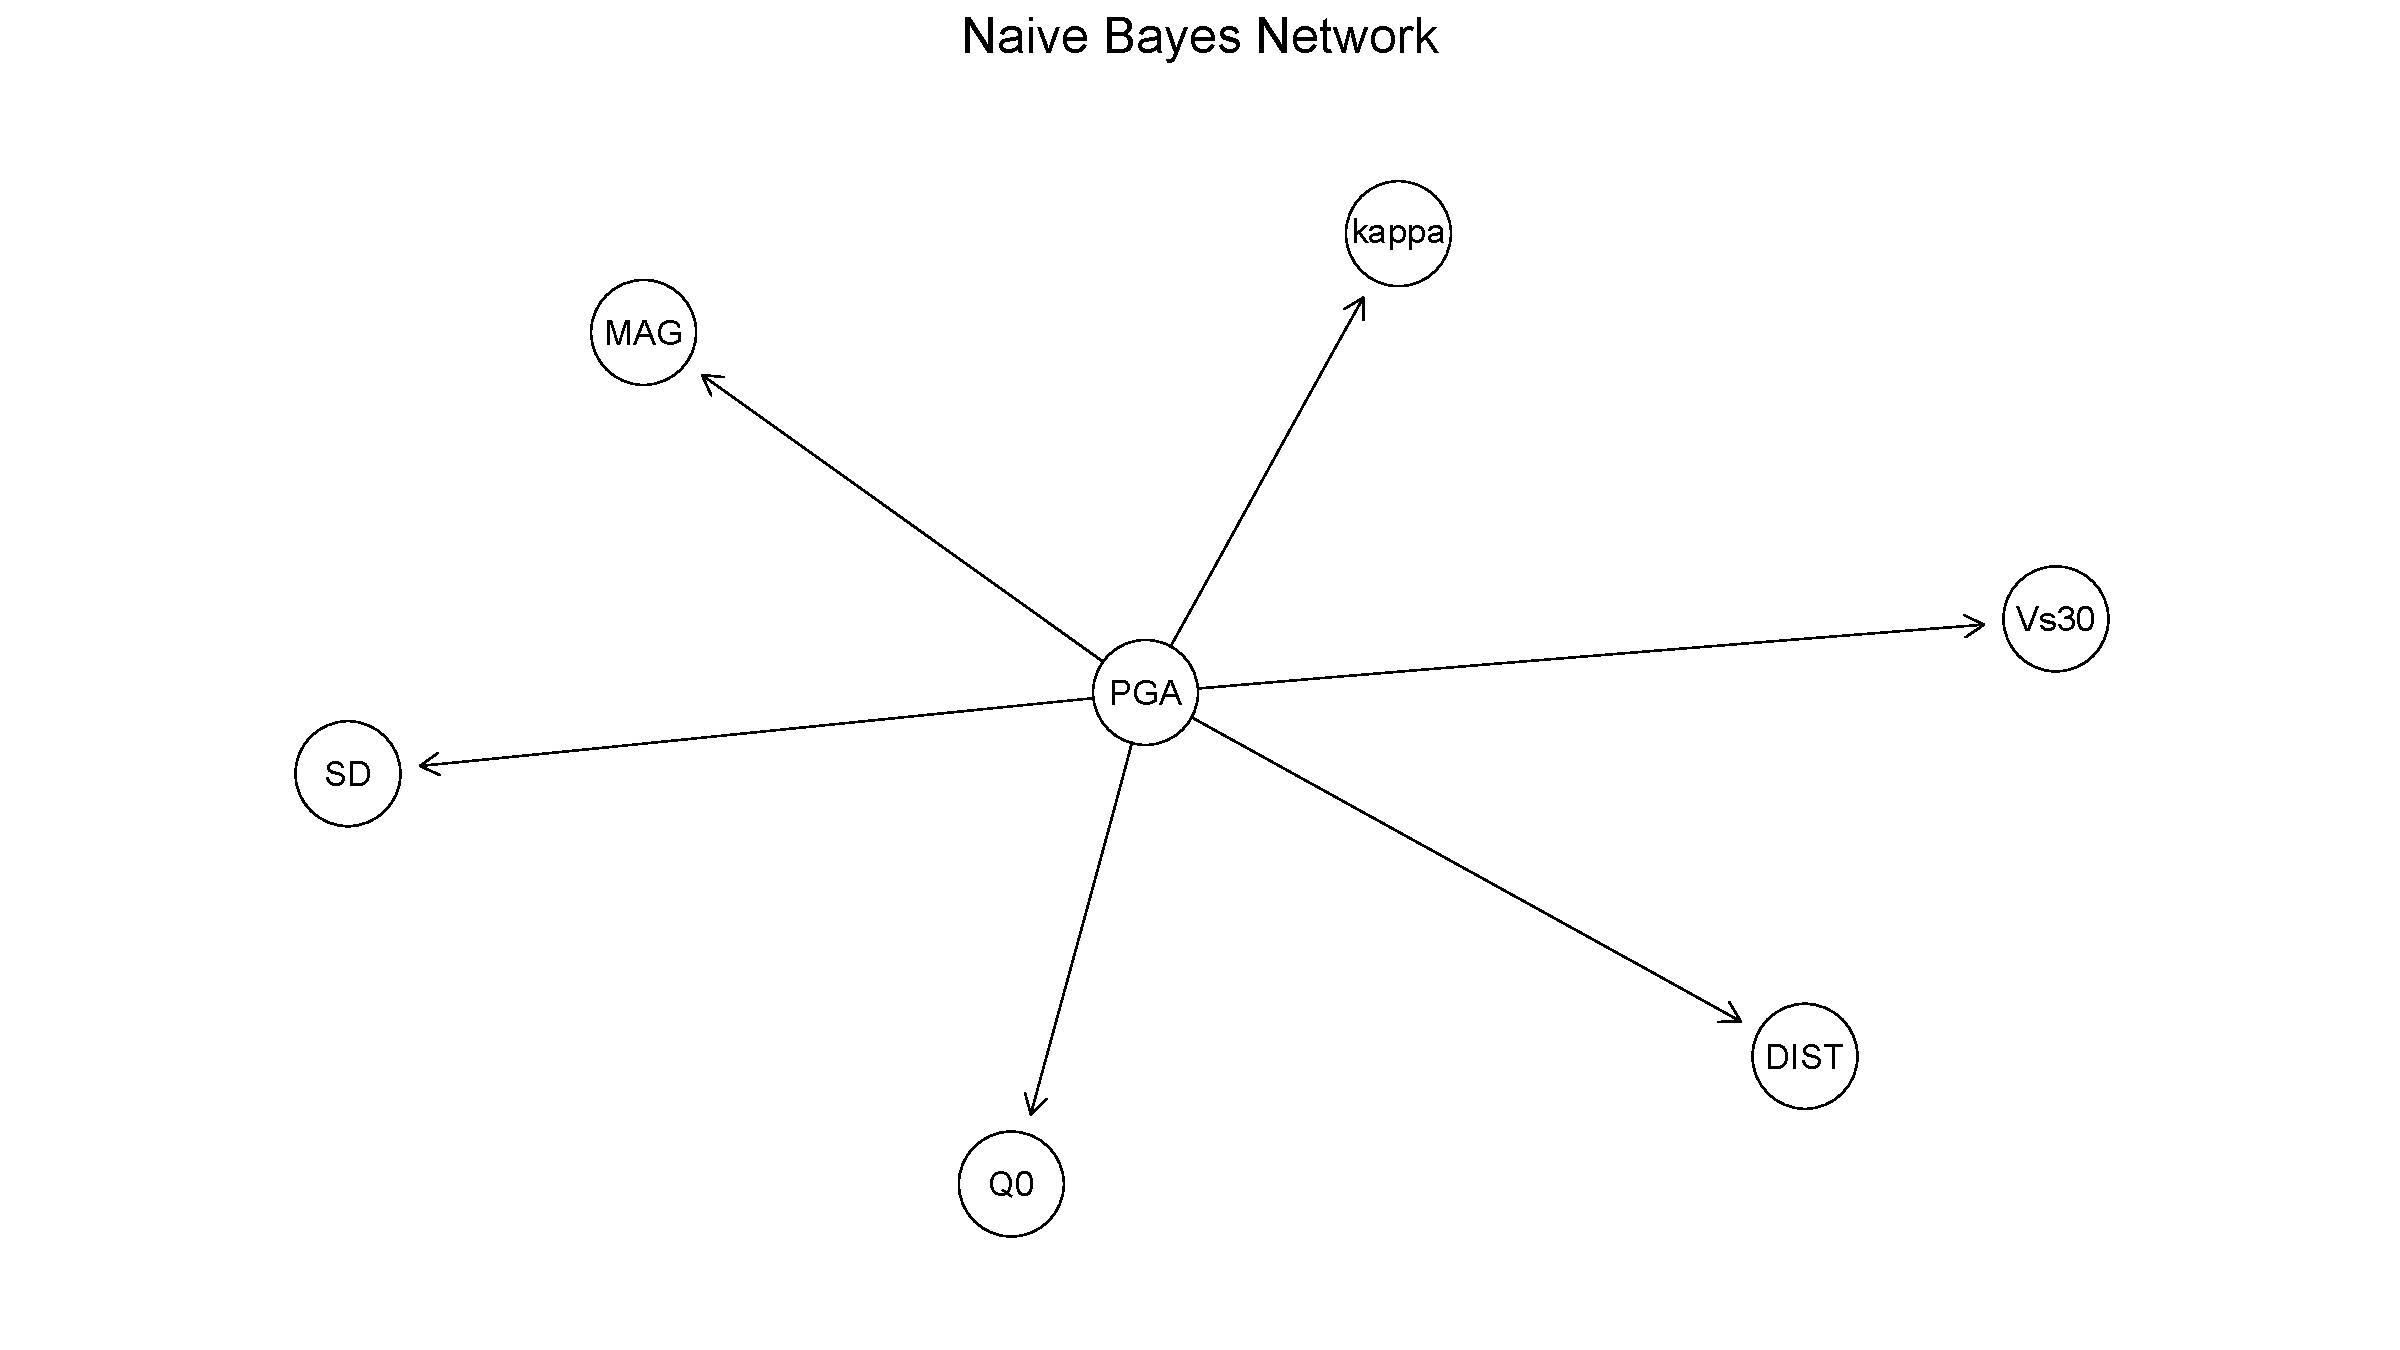
\includegraphics[scale=0.33]{Figures/naive.pdf}
		\rule{35em}{0.5pt}
	\caption[Naive Bayes Network]{A naive Bayes Network of the variables.}
	\label{fig:naive}
\end{figure}
\newpage

Another way of setting up the structure of a Bayesian Network is to rely on expert judgment to define the dependencies between the variables. This is called a causal network since one tries to capture the causal relationships in choosing the dependencies. For the case of predicting PGA from a set of explanatory variables the following causal network(Figure~\ref{fig:causal}) can be reasoned. \\

\begin{figure}[!h]
	\centering
		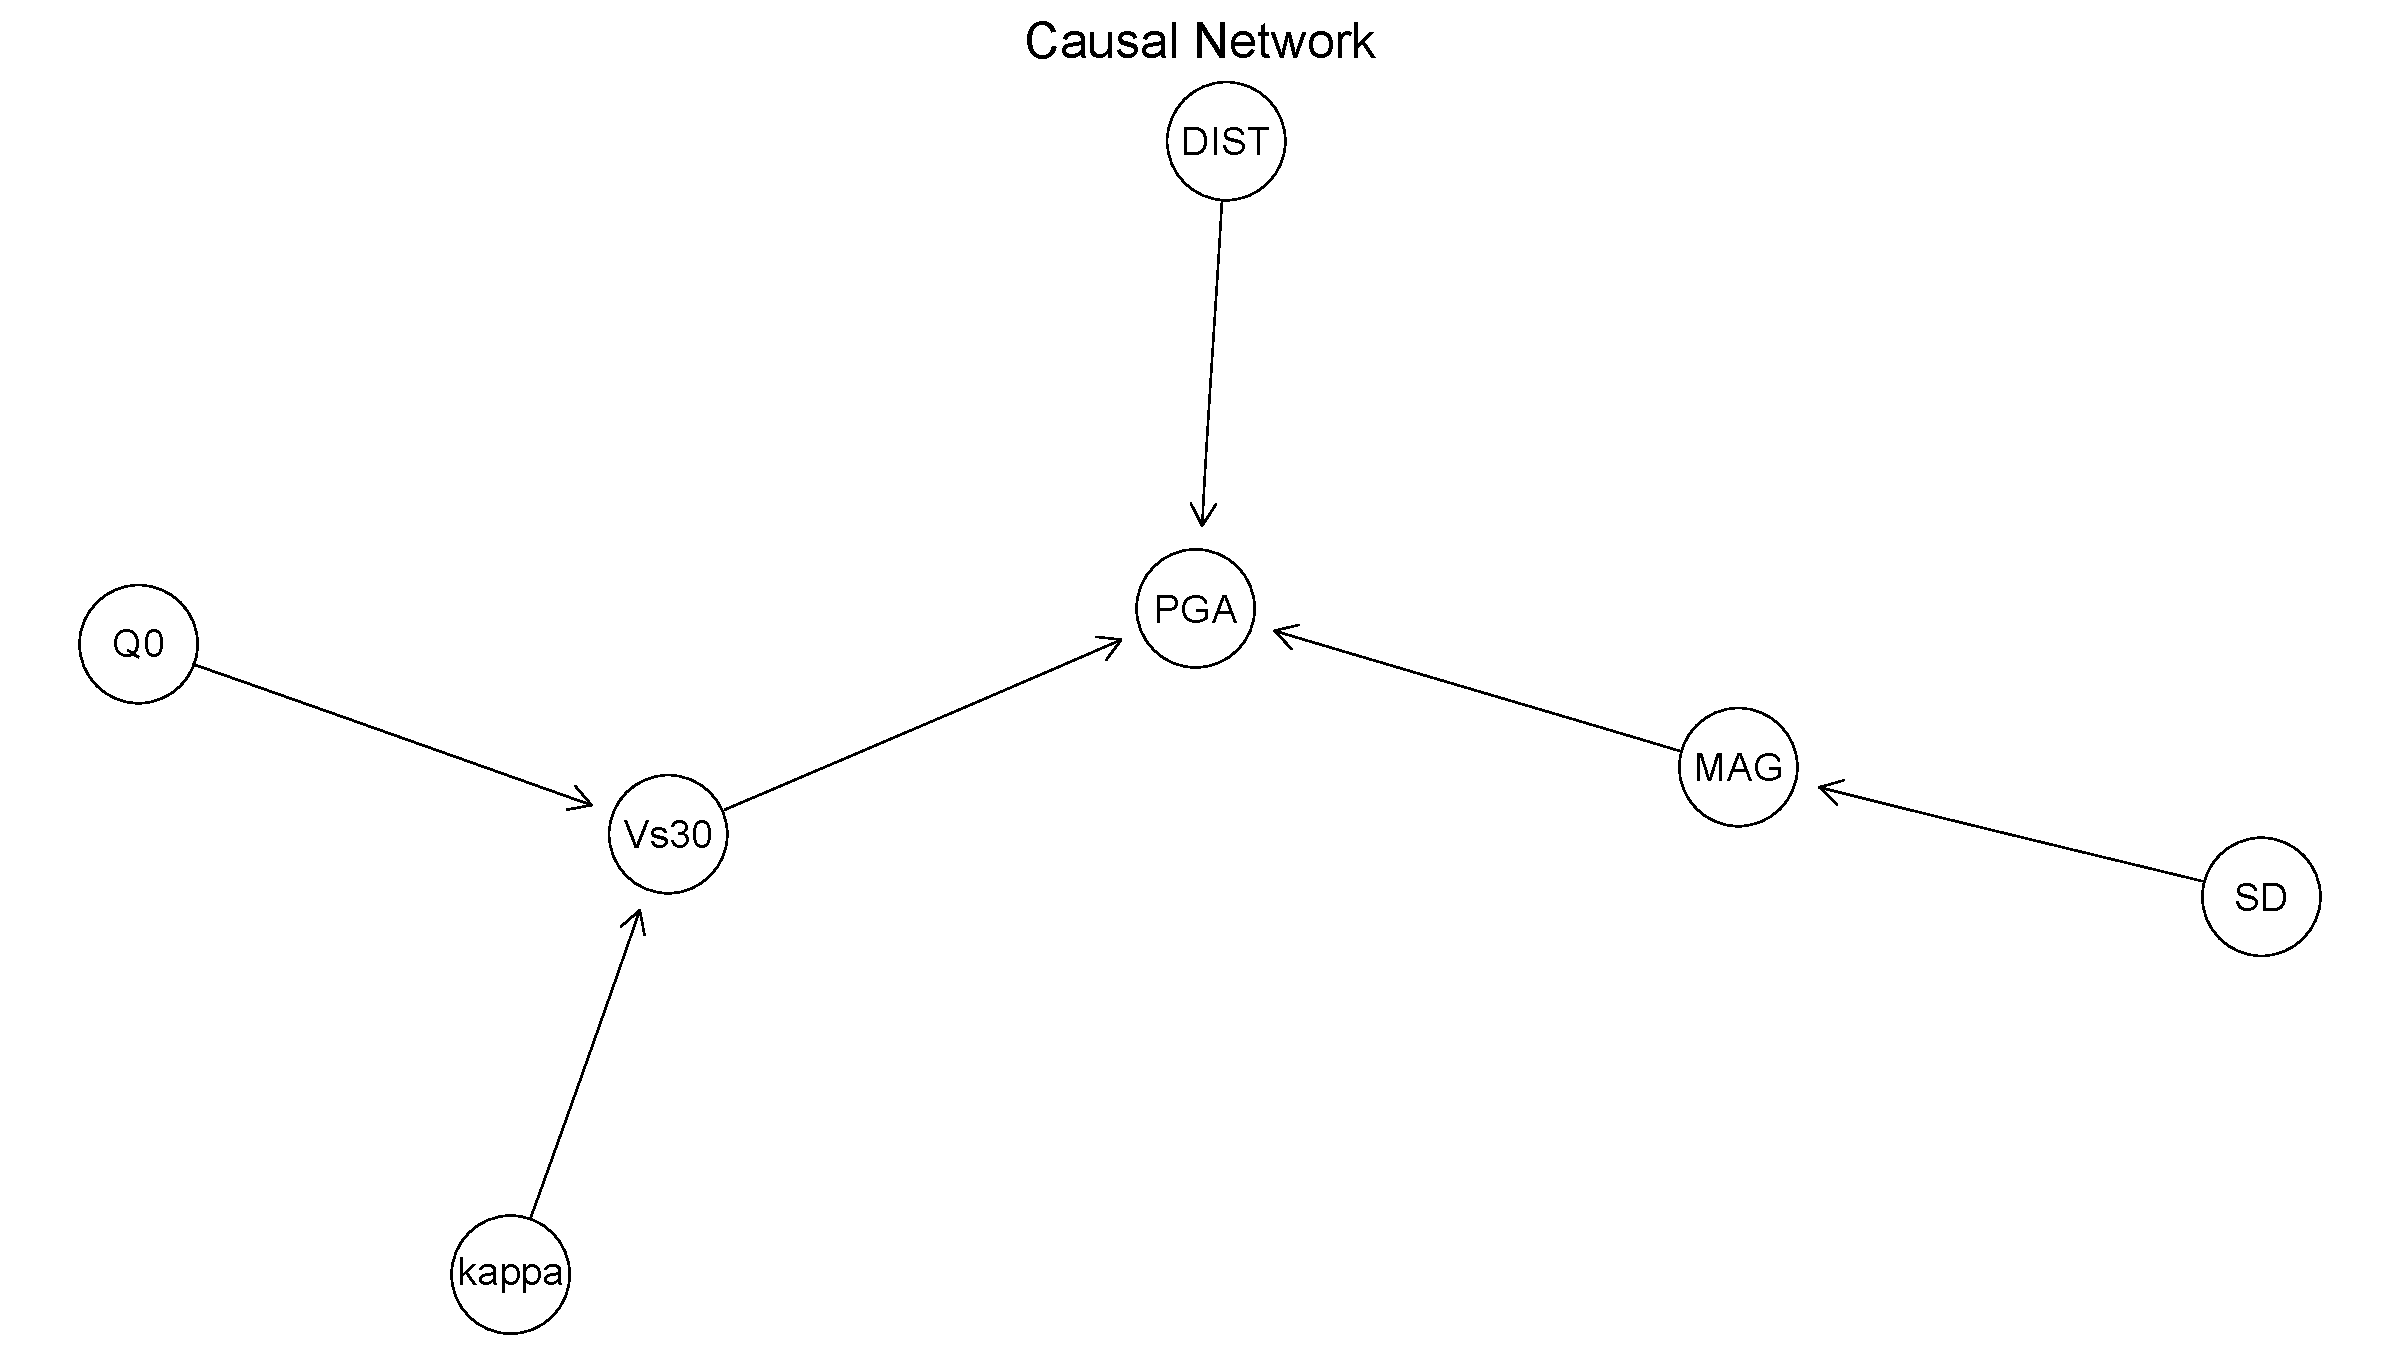
\includegraphics[scale=0.33]{Figures/causal.pdf}
		\rule{35em}{0.5pt}
	\caption[Causal Network]{A causal network representing the beliefs in dependency based on expert knowledge.}
	\label{fig:causal}
\end{figure}

One can argue that the attenuation behavior in deep layer (Q0) is independent from the one in shallow layers (kappa) because this difference reflects the varying materials and environment conditions. Nevertheless, since both are material properties they can influence the shear wave velocity in the first 30m ($V_s30$). One can imagine??.  The distance from the source (DIST) doesn't seem dependent on any other explanatory variable because one can imagine having the same earthquake but choosing a different location on the earth's surface. Moment magnitude (MAG) and stress drop (SD) are dependent since they both refer to the energy that is released during an earthquake. Since the moment magnitude is proportional to the ruptured area the same value can be achieved by a wide range of possible combinations in the ruptures' width and length. This is the reason why it is dependent on the stress drop.\\
One could also have had a look at the data \ref{AppendixA}. Clearly PGA depends on all of the variables but it is also possible to see trend between distance and stress drop, Q0 and, $\kappa_0$ which all seem to decrease exponentially with the distance. But a closer look at the relationship between distance and magnitude shows that there are more datapoints at close distances than at far away points. In the case where one doesn't know the underlying distributions it is always a good idea to consult histograms of the maginal distribution of the variables, too. In this case it is known that stress drop, Q0, $\kappa_0$ and, the distance are all sampled from exponential distributions. That means that the trend in the visualization isn't really there it's just that the dependent variable in the plot is also sampled from an exponential distribution o there are less datapoints at larger values. This can actually been seen in the scatterplots as there are datapoints at large values over the entire range of the independet variable. There are just fewer. This little excourse shows some of the dangers of looking at the data before learning models. One is prone to find patterns, often ones that aren't even there. And for a multidimensional dataset such like this two-dimensional representations always loose some of the information. Sometimes this can't even be avoided by looking at the marginals. On another point, in machine learning there exist the notion of "Data snooping"
\begin{quote}
"If a data set has affected any step in the learning process, its ability to assess the outcome has been compromised. \citep{LearningFromData}"
\end{quote}
From a Bayesian point of view one can say that looking at the data to decide any further steps in the analyses is in itself a step of learning. One goes from a state of ignorance where all hypotheses (in this case the structure of the Bayesian net) have equal probability over to excluding certain hypotheses that don't seem to capture the relationships one has seen. This is essential starting with a uniform distribution as a prior to setting some of the probabilities to zero. The danger is that the model is overfitted and so performs poorly on unseen data. In a Bayesian framework the prior can be thought of as a regularization parameter that guards against overfitting. But for this mechanism to work it is best to have some sort of naive??? prior and not to "fit" the prior on data to have a superb in-sample-error but poor out-of-sample performance.\\
Another way to set up causal networks is to consult literatur about the topic, In the case of Bayesian Networks for ground motion prediction sources could be \cite{kuehn2010} or \cite{Vogel2014}.\\

A third way of defining the structure of a Bayesian network is to learn it from the data itself. Often, not all dependencies between the variables are known and as was seen in causal networks, human domain knowledge can also be misleading and sometimes a strong assumption as it limits the hypothesis space of possible networks vastly. So it is a natural extension to ask whether there are principled ways in the framework of Bayesian networks to let also the structure come from the data. In a sense, according to the Bayesian paradigm, the structure of a network becomes a random variable, too and the task is to jointly estimate the parameters and the structure from the data. In the scope of this paper the constraint-based Grow-Shrink algorithm~\citep{margaritis2003} and the score-based hill-climber are explored.\\
Constraint-based algorithms perform independence tests between the random variables and then set up a network according to the found independencies. The task is therefore one of finding the best minimal I-map. An I-map or independence map is a graph whose independence statements hold for the probability distribution one tries to model. In the case where the graph captures all independence statements this is a perfect I-map. A minimal I-map is graph that is rendered not an I-map anymore by the removal of one edge. This is an important definition because the complete graph over a set of random variables is also an I-map but does not reveal any independencies and therefore carries parameters that are redundant.In practice one doe not find one single best minimal I-map but a class of graphs that carry the same independence statements and are therefore called I-equivalent~\citep{koller2009}. 
The Grow-Shrink algorithm tries to construct the structure of a network by finding the Markov Blankets of the variables. A Markov Blanket of one variable is a set of variables that renders that variable to be d-separated from all other variables. That means that knowing the state of any variable that is not in the Markov Blanket has no effect on knowing the state of the variable in interest. One could say that the Markov Blanket "shields" a variable from the influence of all other variables. Graphically it is the set of parents, children and parents of the children of the variable in interest~\citep{koller2009}. In the Growing phase of the Grow-Shrink algorithm independence tests between variables are performed which are the basis to decide if a variable should be included in the Markov blanket. These test occur given the state of the Markov Blanket. Depending on the initial ordering of the variables this can lead to include redundant variables in the Markov Blanket which are subsequently removed by the independence test of the Shrinking phase~\citep{margaritis2003}. For learning the structure of a Bayesian network according to the Grow-Shrink algorithm the mutual information (Equation~\ref{eqn:mutual}) is used as an independence test.

\begin{equation}
I(X;Y) = \sum_{y \in Y} \sum_{x \in X} 
                 p(x,y) \log{ \left(\frac{p(x,y)}{p(x)\,p(y)}
                              \right) }, \,\! 
\label{eqn:mutual}
\end{equation}

 It estimates the dependence between two variables by comparing the joint distribution to the product of the marginal distributions, since in the case of independence the joint distribution factorizes to the product of the marginal distribution. From a Venn-diagram point of view it calculates the area shared by two distribution relative to the total area of the distributions.\\
The learned network is visualized in Fig.\ref{fig:gs}. It is interesting to see that there are no direct dependencies between the explanatory variables. Even more the variable $V_s30$ is completely ignored. By comparing this result to work of~\citep{Vogel2014}which uses a similar data set( ;) ) one can find that this seems to be a consistent result when learning the structure of a Bayesian network for ground motion prediction from data. One causal reason might be that $V_s30$ is merely a proxy in quantifying the capability of the soil to amplify the amplitudes of seismic waves. One should keep in mind that the data was generated by the stochastic model of Boore~\citep{boore2003} and that a number of samples is not the full distribution.\\
\begin{figure}[htbp]
	\centering
		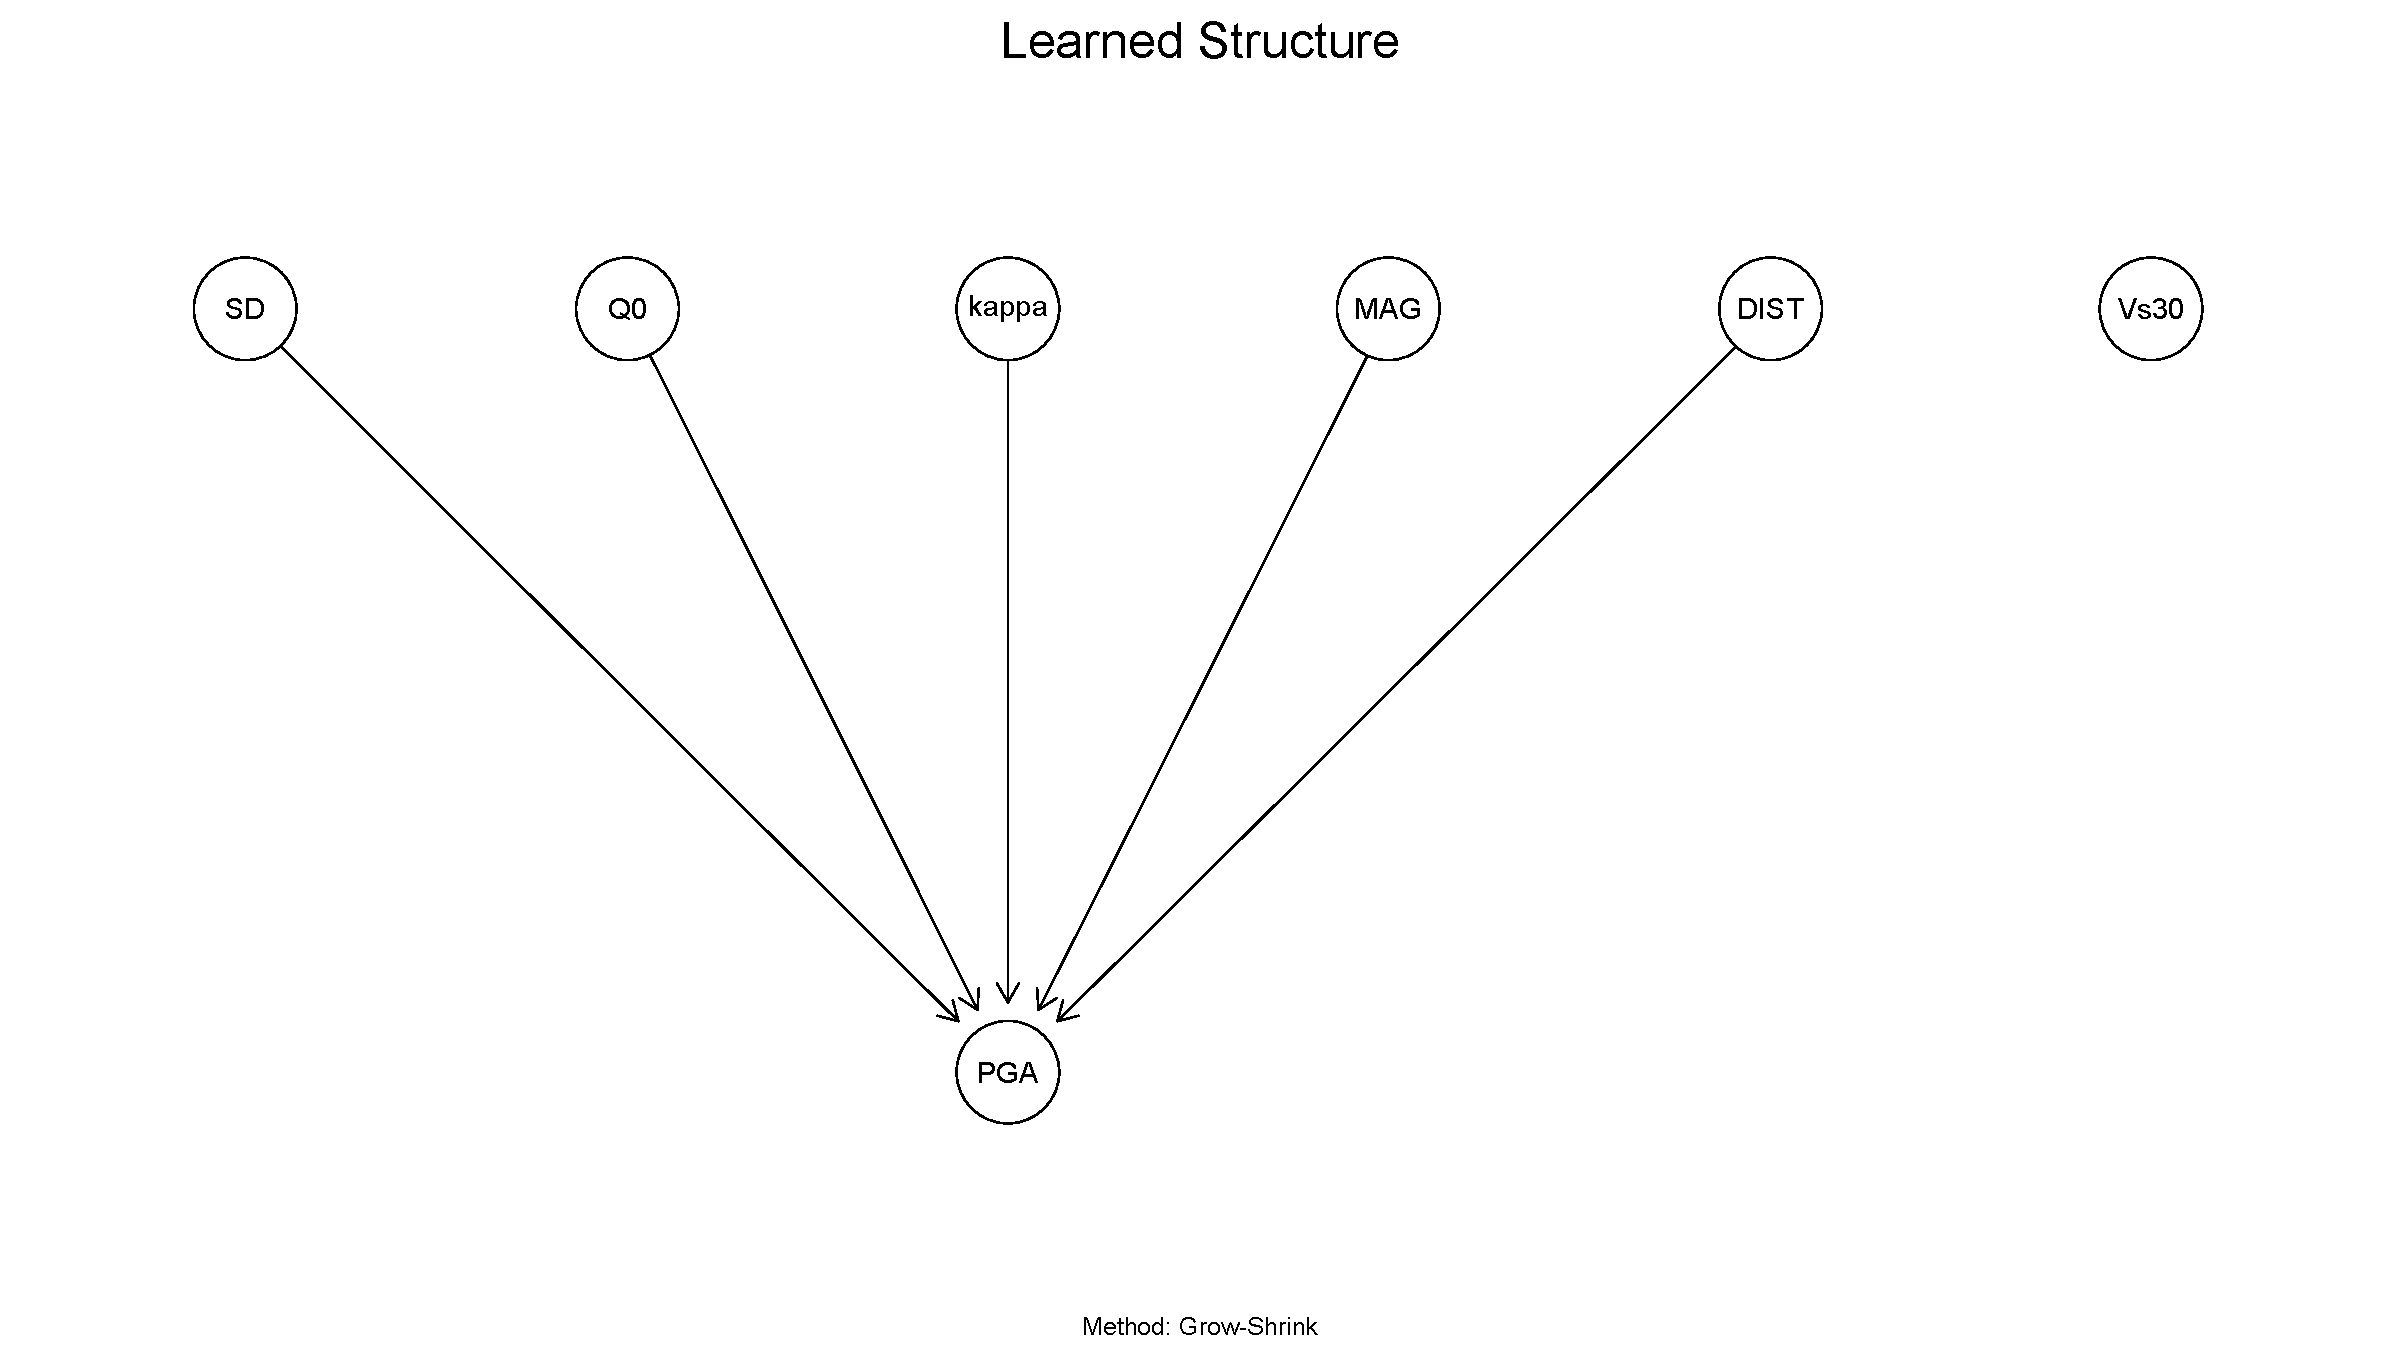
\includegraphics[scale=0.33]{Figures/gs_one.pdf}
		\rule{35em}{0.5pt}
	\caption[Contraint-based Grow-Shrink Network]{gs}
	\label{fig:gs}
\end{figure}

Score-based algorithms view the problem of finding the structure of a Bayesian network from an optimization point of view. In contrast to the constraint-based algorithms, score-based ones do not try to construct the structure from information about single connections between variables but take the network as a whole, compute a score that measures how well the current structure fit the data and, try to find the network that maximizes that score. Consequently, score-based algorithm pose a search problem in the space of possible network structures. Depending on the number of variables and the underlying probability distribution in most cases this is a NP-hard problem and requires some approximation techniques~\citep{koller2009}. \\
A Hill-climber can be thought of as the opposite of gradient descent since it tries to maximize a predefined score, most commonly a likelihood measure that estimates the probability of the data been generated by the given structure, in contrast to minimizing an error term. For the construction of a Bayesian network using the hill-climber algorithm a score consisting of the is the maximized likelihood L (Equation \ref{eqn:likelihood}) that gives the probability of the data being generated by the graph G and the parameters $\theta$ and the Bayesian Information Criterion (BIC) (Equation~\ref{eqn:BIC}~\citep{schwarz}) as a regularization term consisting of the number of free parameters $k$ and the size of the data $n$ is used.

\begin{equation}
L = \operatorname*{arg\,max}_\theta P(x\mid \theta, G)
\label{eqn:likelihood}
\end{equation}

\begin{equation}
BIC = -2*ln L + k* ln(n)
\label{eqn:BIC}
\end{equation}


\begin{figure}[htbp]%
	\centering
		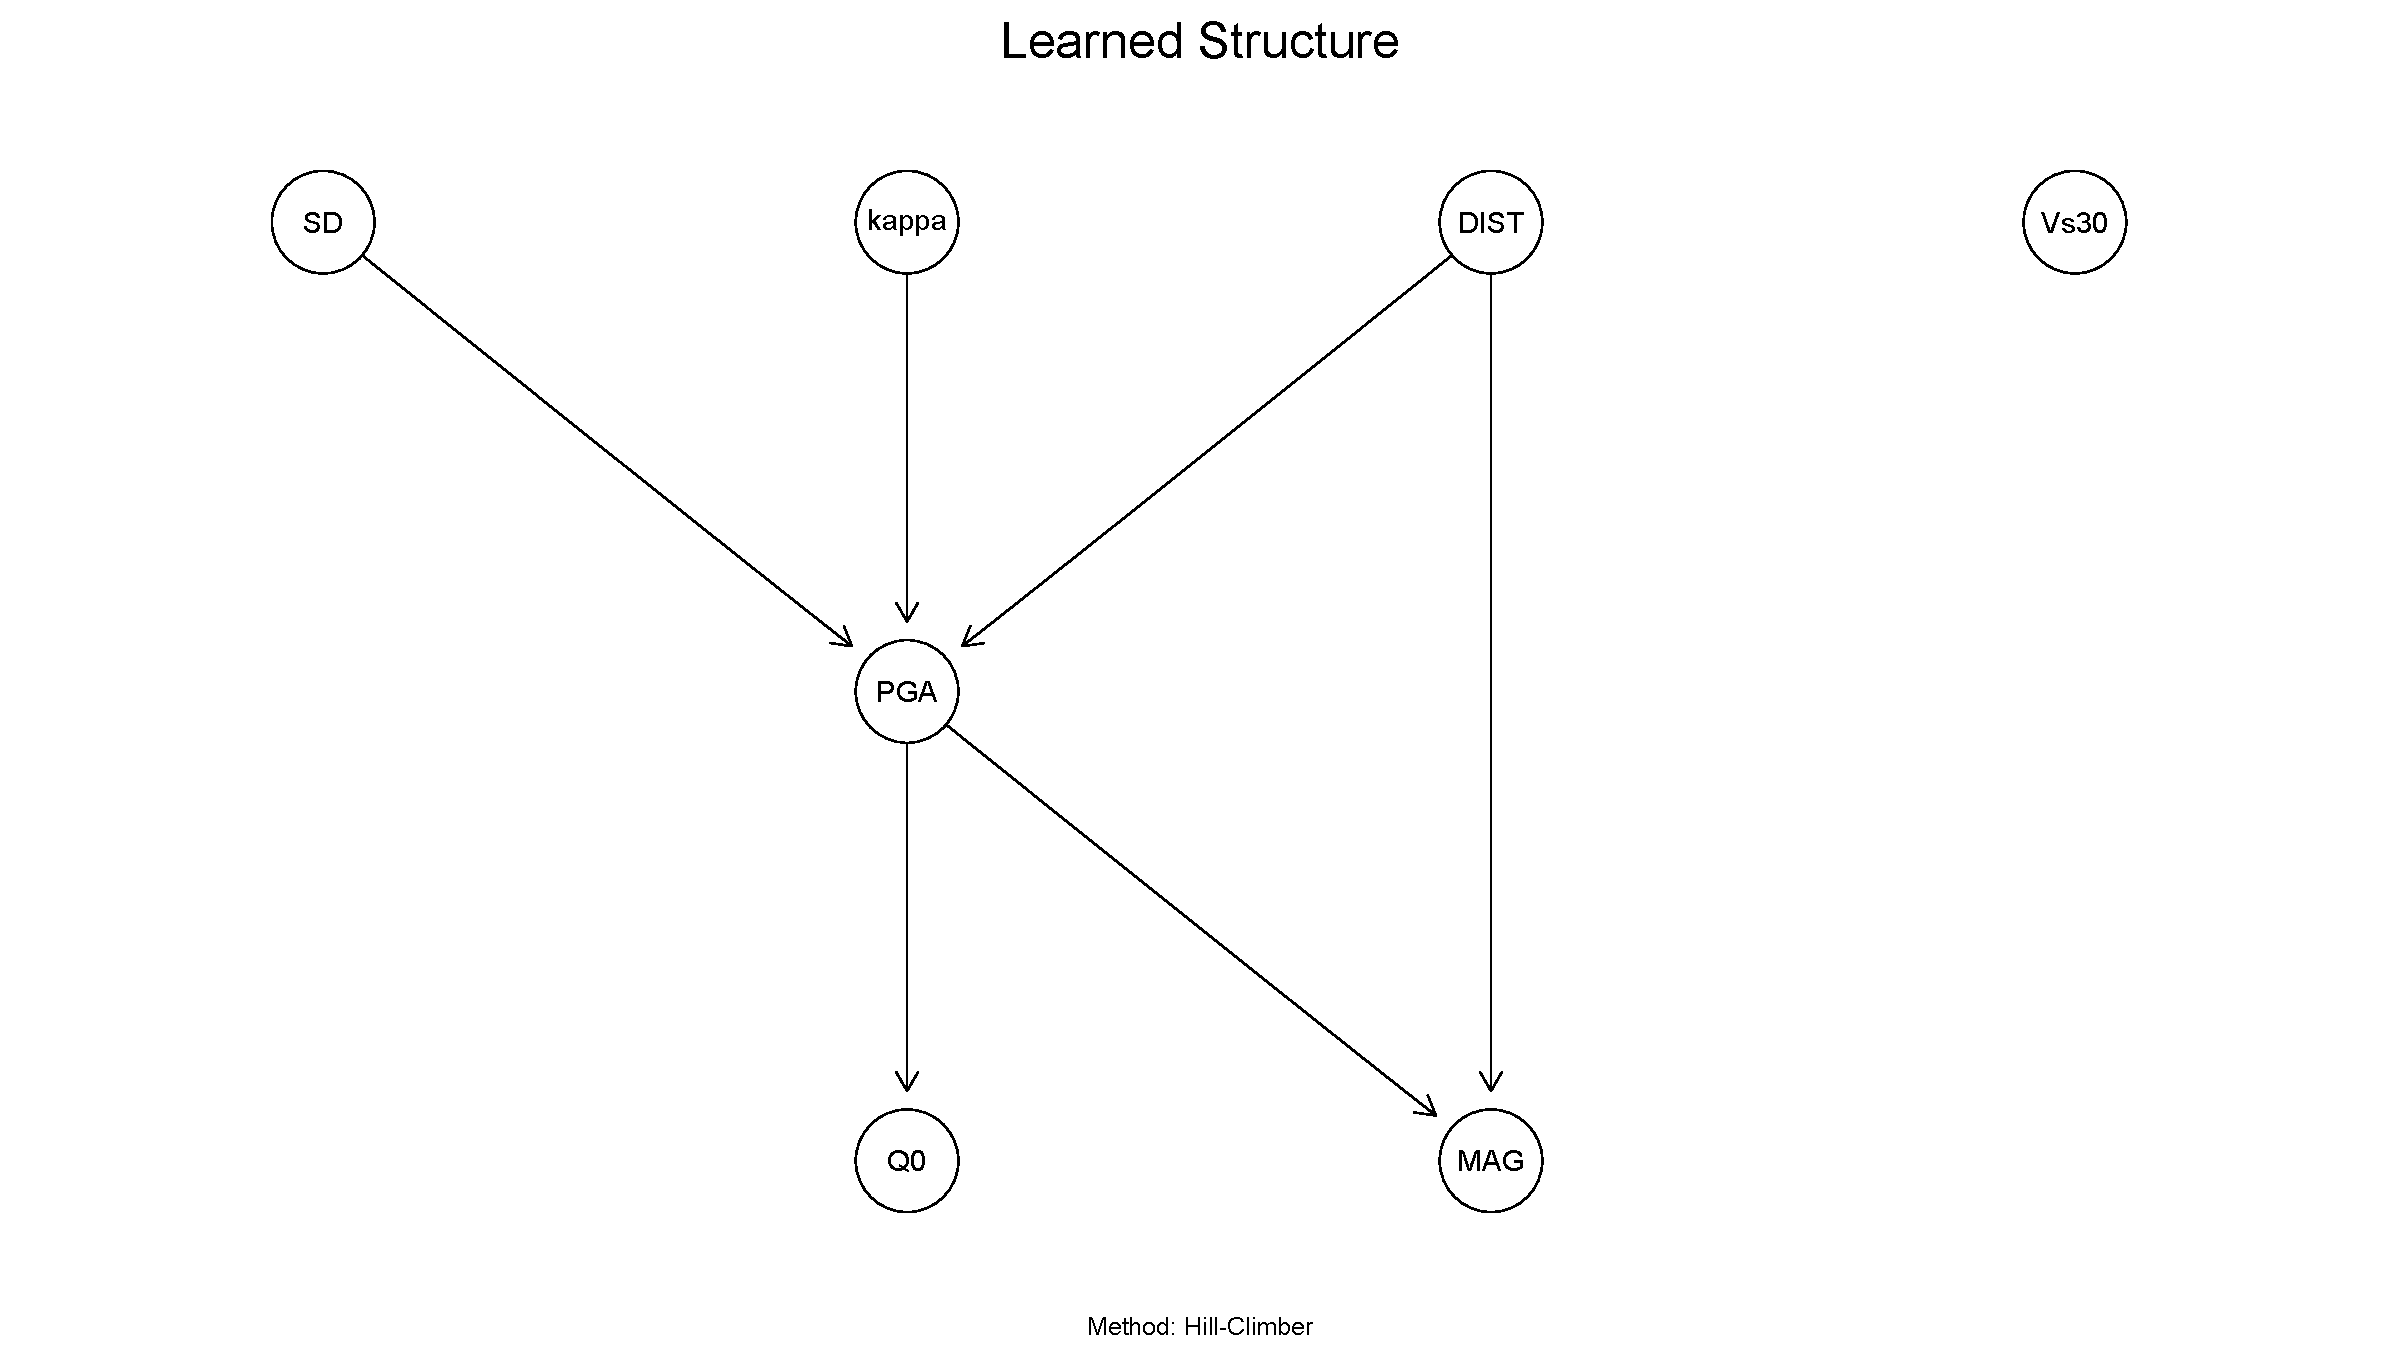
\includegraphics[scale=0.33]{Figures/hc_one.pdf}
		\rule{35em}{0.5pt}
	\caption[Score-based Hill-Climber Network]{hc}
	\label{fig:hc}
\end{figure}

there is a third. bayes model averaging. create ensemble of nets and average the predictions.
The learned structure networks look pretty similar. Compare to \citep{Vogel2014} because they are from similar data. Actually a series of networks was learned: \ref{AppendixA} \ref{AppendixB}

%----------------------------------------------------------------------------------------

\section{Parameter Learning}

bayesian parameter estimation
%----------------------------------------------------------------------------------------

 
% Chapter 1

\chapter{Testing} % Main chapter title

\label{Chapter3} % For referencing the chapter elsewhere, use \ref{Chapter1} 

\lhead{Chapter 3. \emph{Testing}} % This is for the header on each page - perhaps a shortened title

Testing the outcomes of a model is an integral part of modeling dependencies since it gives a handle to tell how good the reality can be approximated.
For doing so, many different measures and methodologies have been developed, all targeting a different part of the question what a "good" model should be. There are measures like the mean squared error and the mean absolute error that quantify the difference between the observed data points and the values predicted from the model. These can be thought of as in-sample error metrics since the data to construct the model is also used to estimate the error. Intuitively, this seems like a good idea because the data is all one has to construct a model and therefore the best fit has the highest probability of producing consistent results. In reality, this can cause a phenomenon called "overfitting" where the model is so much adjusted to the data that it has a low in-sample error but performs poorly on unseen data. This cane even lead to the conviction that some of the data has to be excluded because the worsen the fit.
There is a difference between function approximation and learning a model. In function approximation the goal is to estimate the parameters of a model so that the final function matches the given data the closest. In learning a model the underlying dependencies are usually not known and the data only represent a subset of the whole range of possible values, often including some noise. Hence, the task in learning a model is to match the model complexity  to the data resources~\citep{LearningFromData}. Particular in a scenario of estimating natural hazard it would be desirable to have a measure that can tell from a sample of data points something about how the model might behave predicting on unseen data.\\

%----------------------------------------------------------------------------------------

\section{Learning and Test set}
One common approach to get a handle of a models' out-of-sample or prediction performance is to divide the data from which the models parameters should be estimated into a learning or training data set and a test data set. Then the learning data is used to estimate the parameters and the models performance is tested on the test data set. This has the effect of simulating unseen data since the test data has not been used for learning the models parameters.

\begin{table}[h]
\centering
\begin{tabular}{ l l l l l  }
 \hline
  & \multicolumn{4}{c}{error measure} \\
 \hline
 net & mean & median & mode & probability\\
 \hline
 causal   & 4.816    & 4.933  & 9.739   &-1.772\\
 naive   & 1.488      & 1.801 & 1.937  &-1.35\\
 hill-climber   & 1.068      & 1.339 & 1.503  &-1.016\\
 grow-shrink   & 0.844     & 1.124  & 1.149 &-0.874\\
\end{tabular}
\caption[Validation Error]{error measures}
\label{tab:2}
\end{table}
%----------------------------------------------------------------------------------------

\section{Crossvalidation}

\begin{table}[h]
\centering
\begin{tabular}{ l l l l l  }
 \hline
  & \multicolumn{4}{c}{error measure} \\
 \hline
 net & mean & median & mode & probability\\
 \hline
 causal   & 4.904    & 5.066  & 9.421   &-1.764\\
 naive   & 1.482      & 1.703 & 1.762  &-1.342\\
 hill-climber   & 1.041      & 1.488 & 1.503  &-1.017\\
 grow-shrink   & 0.823     & 1.202  & 1.149 &-0.875\\
 
\end{tabular}
\caption[Crossvalidation Error]{error measures}
\label{tab:3}
\end{table}
%----------------------------------------------------------------------------------------

\section{Bias and Variance Decomposition}

\begin{table}[h]
\centering
\begin{tabular}{ l l l l }
 \hline
 & \multicolumn{3}{c}{error measure} \\
 \hline
 net & mean & median & mode\\
 \hline
 causal & 4.876 & 5.007 & 9.233\\
 naive & 1.472 & 1.682 & 1.709\\
 hill-climber & 1.029 & 1.341 & 1.478\\
 grow-shrink & 0.786 & 1.115 & 1.152\\
\end{tabular}
\caption[Bias]{error measures}
\label{tab:4}
\end{table}

\begin{table}[h]
\centering
\begin{tabular}{ l l l l }
 \hline
  & \multicolumn{3}{c}{error measure} \\
 \hline
 net & mean & median & mode\\
 \hline
 causal & 0.01& 0.185 & 1.661\\
 naive & 0.0091 & 0.136 & 0.546\\
 hill-climber & 0.0032 & 0.0694 & 0.128\\
 grow-shrink & 0.003 & 0.0622& 0.092\\
\end{tabular}
\caption[Variance]{error measures}
\label{tab:5}
\end{table}
% Chapter 4

\chapter{Conclusions} % Main chapter title

\label{Chapter4} % For referencing the chapter elsewhere, use \ref{Chapter1} 

\lhead{Chapter 1. \emph{Introduction}} % This is for the header on each page - perhaps a shortened title
The following  work deals with the problem of seismic hazard assesment.
 


%----------------------------------------------------------------------------------------
%	THESIS CONTENT - APPENDICES
%----------------------------------------------------------------------------------------

\addtocontents{toc}{\vspace{2em}} % Add a gap in the Contents, for aesthetics

\appendix % Cue to tell LaTeX that the following 'chapters' are Appendices

% Include the appendices of the thesis as separate files from the Appendices folder
% Uncomment the lines as you write the Appendices

% Appendix A
\chapter{Additional Figures}

\newpage
\section{Folds of Learned Networks: Hill-Climber} % Main appendix title

\label{AppendixA1} % For referencing this appendix elsewhere, use \ref{AppendixA}

\lhead{Appendix A.1 \emph{Folds of Learned Networks: Hill-Climber}} % This is for the header on each page - perhaps a shortened title
\begin{figure}[!htbp]%
	\centering
		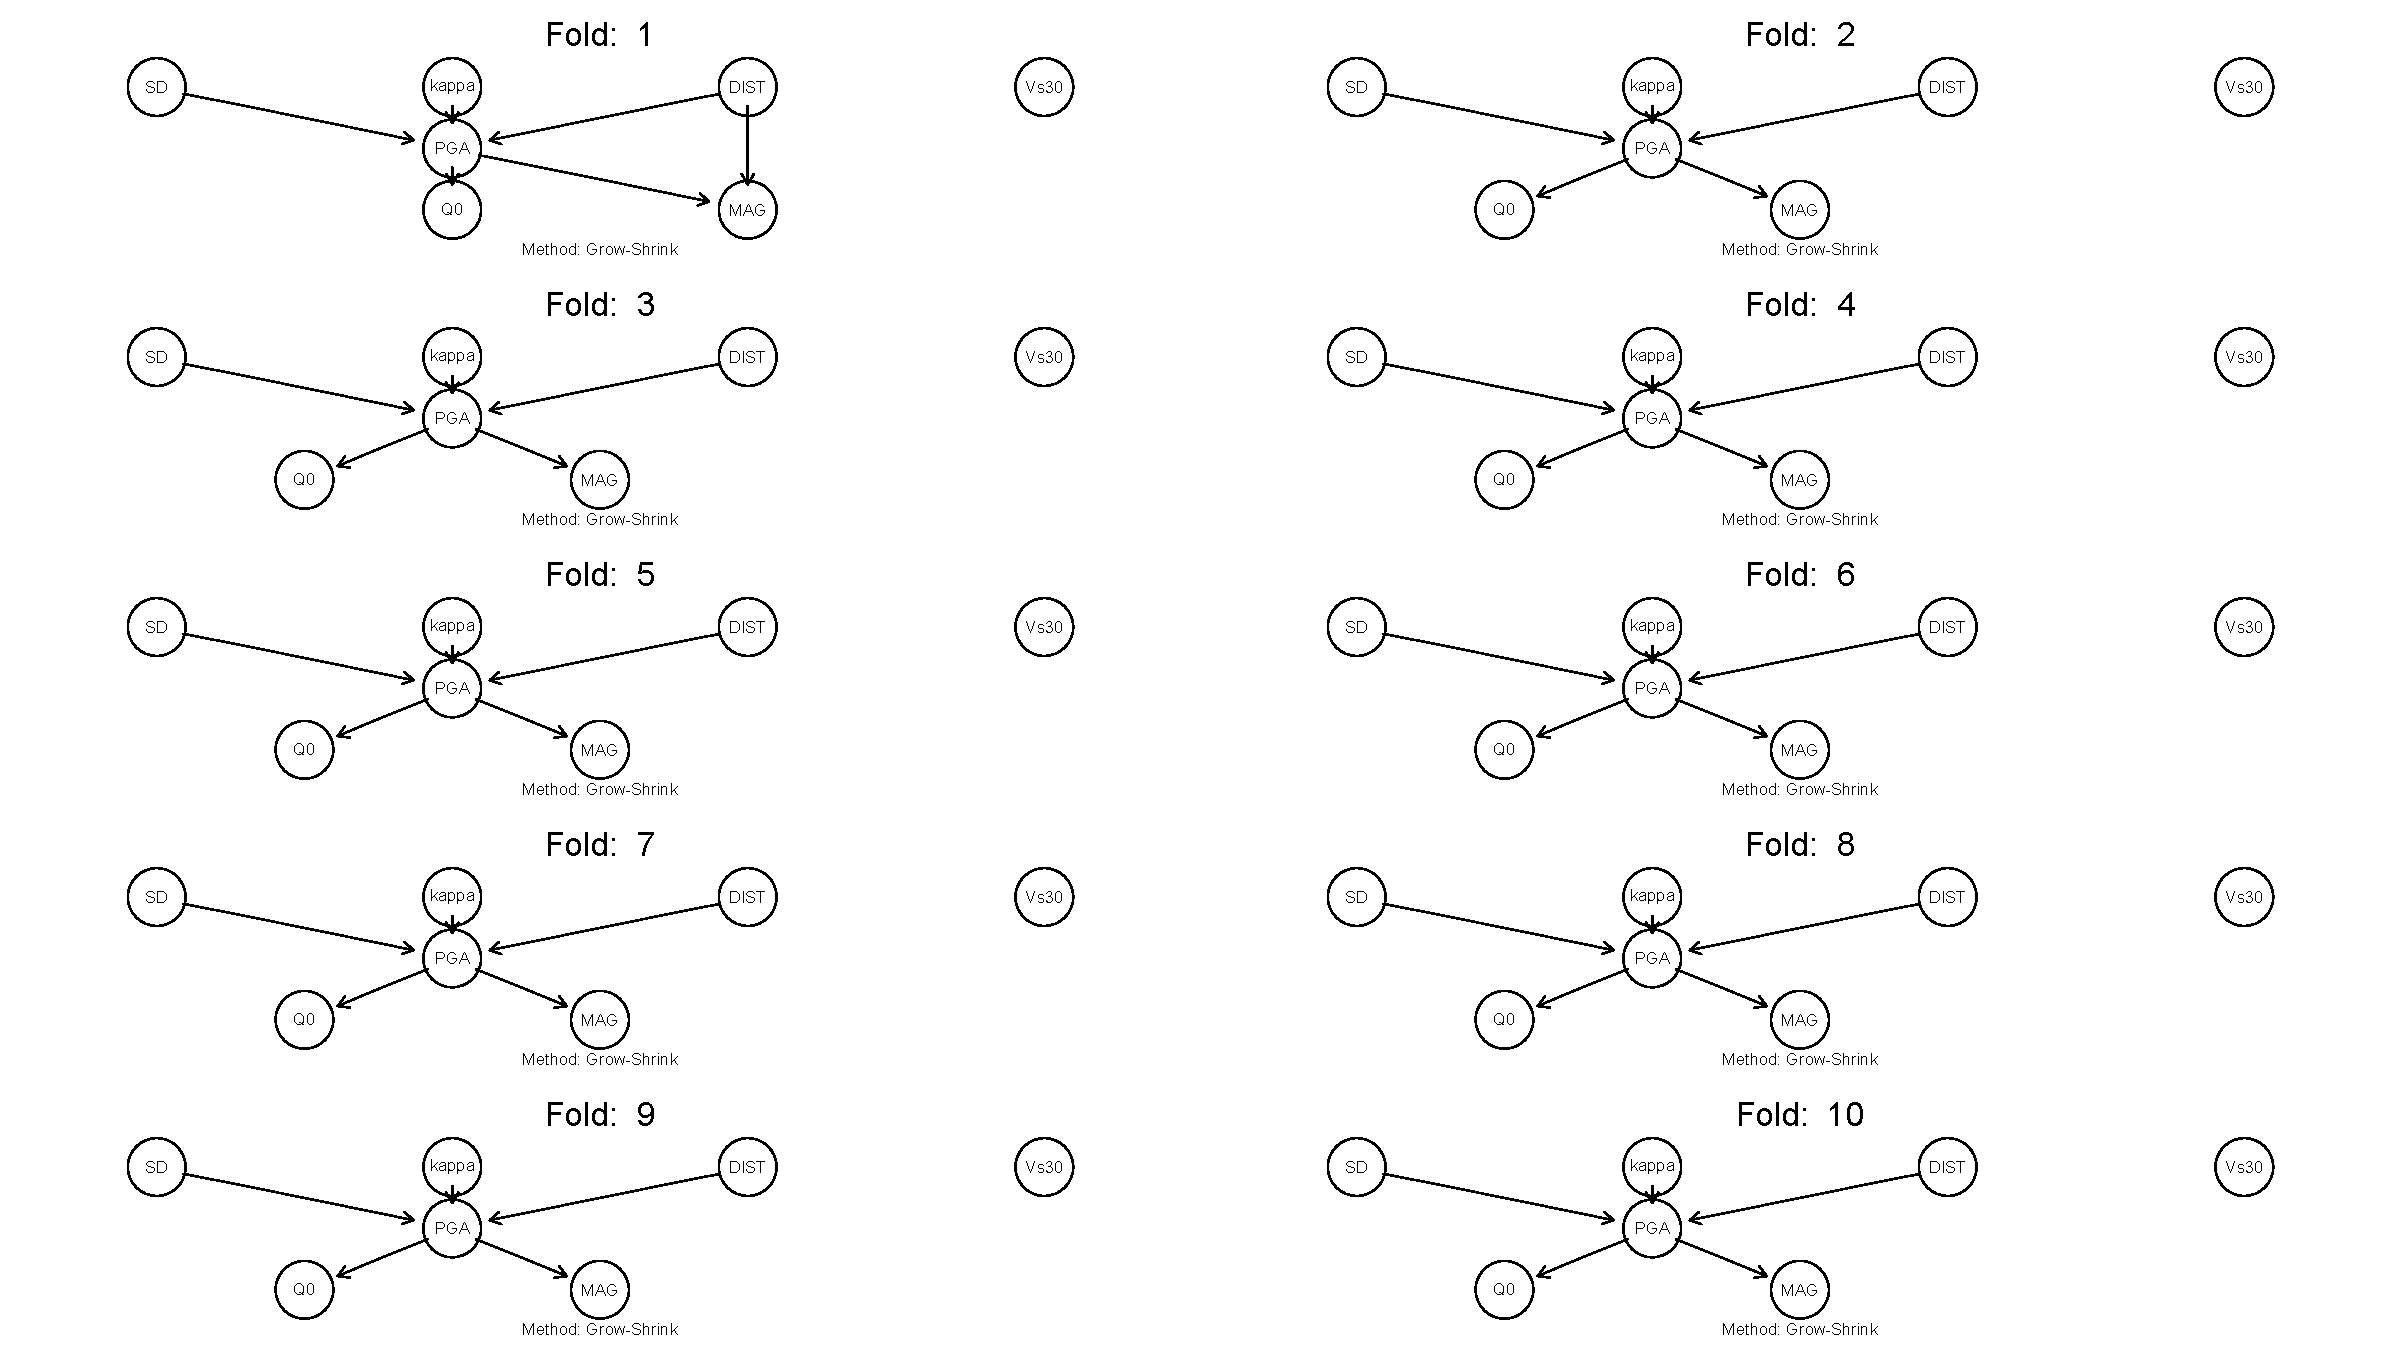
\includegraphics[angle=90,scale = 0.5]{Figures/hc.pdf}
		\rule{35em}{0.5pt}
	\caption*{Folds of Learned Networks: Hill-Climber}
\end{figure}

\newpage
\section{Folds of Learned Networks: Grow-Shrink} % Main appendix title

\label{AppendixA2} % For referencing this appendix elsewhere, use \ref{AppendixA}

\lhead{Appendix A.2 \emph{Folds of Learned Networks: Grow-Shrink}} % This is for the header on each page - perhaps a shortened title
\begin{figure}[!htbp]%
	\centering
		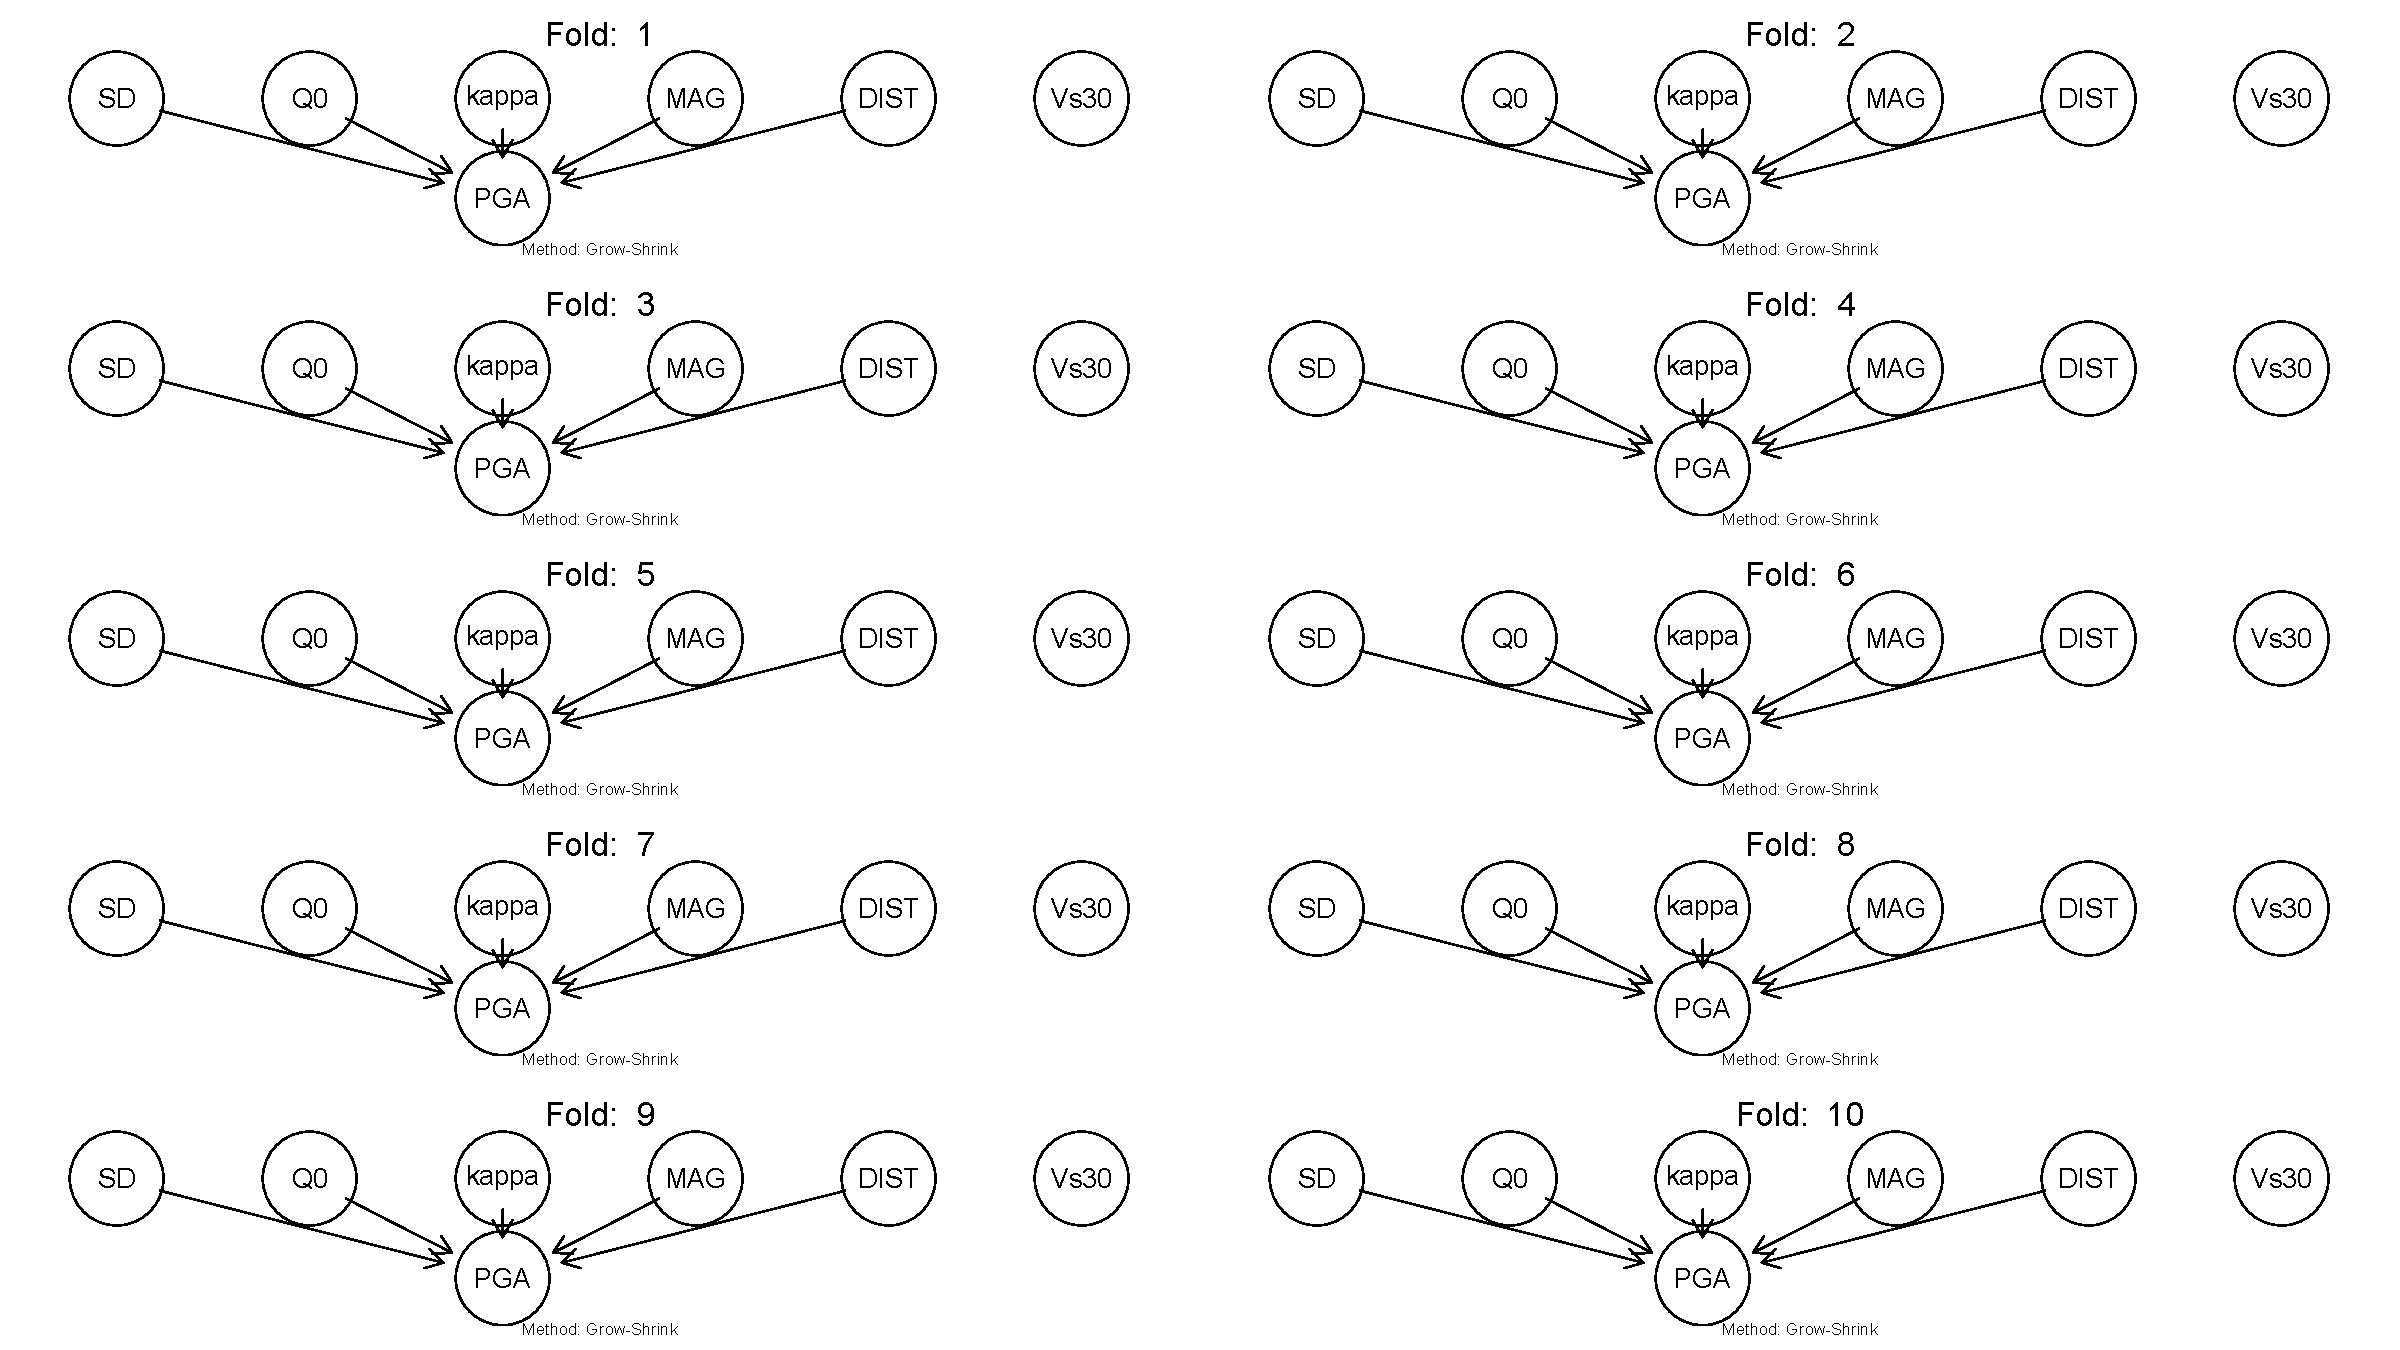
\includegraphics[angle=90,scale=0.5]{Figures/gs.pdf}
		\rule{35em}{0.5pt}
	\caption*{Folds of Learned Networks: Grow-Shrink}
\end{figure}

\addtocontents{toc}{\vspace{2em}} % Add a gap in the Contents, for aesthetics

\backmatter

%----------------------------------------------------------------------------------------
%	BIBLIOGRAPHY
%----------------------------------------------------------------------------------------

\label{References}

\lhead{\emph{References}} % Change the page header to say "Bibliography"

\bibliographystyle{apa} % Use the "unsrtnat" BibTeX style for formatting the Bibliography

\bibliography{References} % The references (bibliography) information are stored in the file named "Bibliography.bib"

\end{document}  